\subsection{Vorbereitende Experimente}
\subsubsection{Resonanzfrequenz}
In Abbildung \ref{fig:zwei-resonanzen} sind die Differenzen der aufeinanderfolgenden Resonanzfrequenzen
aus Tabelle \ref{tab:zwei-resonanzen} gegen die Anzahl von Zylindern aufgetragen. Die Fitfunkton der Form
\begin{align}
    f_\text{diff}(n) &= \frac{c}{2(0.05\cdot n)^a}
    \intertext{nach \eqref{eqn:resonanzfrequenz} führt zu den Parametern}
    \input{build/50mm-zwei-resonanzen.tex}
    \;.
\end{align}

\begin{figure}
    \centering
    \includegraphics[width=0.8\textwidth]{build/50mm-zwei-resonanzen.pdf}
    \caption{Differenz der Resonanzfrequenzen aufgetragen gegen die Zylinderanzahl.}
    \label{fig:zwei-resonanzen}
\end{figure}

\begin{table}
    \centering
    \caption{Daten der ersten Messreihe.}
    \label{tab:zwei-resonanzen}
    \pgfplotstabletypeset[
        dec sep align,
        col sep=comma,
        use comma,
        every head row/.style={before row=\toprule, after row=\midrule},
        every last row/.style={after row=\bottomrule},
        columns/0/.style ={column name={Anzahl Zylinder}},
        columns/1/.style ={column name=$f_\text{R,1}\:/\:\si{\kilo\hertz}$},
        columns/2/.style ={column name=$f_\text{R,2}\:/\:\si{\kilo\hertz}$},
        columns/3/.style ={column name=$f_\text{diff}\:/\:\si{\kilo\hertz}$},
    ]{build/50mm-zwei-resonanzen.csv}
\end{table}

\FloatBarrier

\subsubsection{Messung mit dem Computer}
In Abbildung \ref{fig:50mm-oszi-computer-01} sind die Daten der Messung an einem Zylinder im Frequenzbereich von
$1$~bis~$\SI{10}{\kilo\hertz}$ zu sehen, einmal als Oszilloskopbild, einmal als Plot der Computermessung.

\begin{figure}[ht]
    \centering
    \begin{subfigure}{0.49\textwidth}
        \centering
        \includegraphics[width=\textwidth]{build/50mm-oszi-computer-01.pdf}
        \caption{Messdaten des Computers.}
        \label{fig:50mm-computer}
    \end{subfigure}
    \begin{subfigure}{0.49\textwidth}
        \centering
        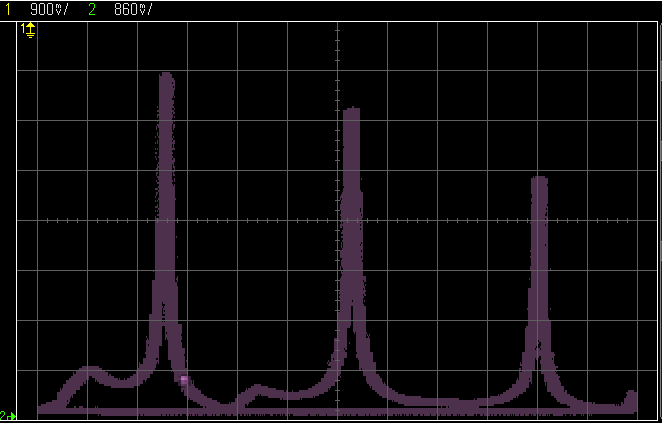
\includegraphics[width=\textwidth]{data/Messaufgabe-2/01zylinder.png}
        \caption{Oszilloskopbild.}
        \label{fig:50mm-oszi}
    \end{subfigure}
    \caption{Messergebnisse für einen Zylinder.}
    \label{fig:50mm-oszi-computer-01}
\end{figure}

In Abbildung \ref{fig:50mm-computer-04-12} ist im Vergleich zu
\ref{fig:50mm-oszi-computer-01}\subref{fig:50mm-computer} gut zu sehen,
dass die Anzahl der Maxima mit der Anzahl der Zylinder ansteigt,
was die Theorie in Gleichung \eqref{eqn:resonanzfrequenz} darlegt.

\begin{figure}[ht]
    \centering
    \begin{subfigure}{0.49\textwidth}
        \centering
        \includegraphics[width=\textwidth]{build/50mm-oszi-computer-04.pdf}
        \label{fig:50mm-computer-04}
    \end{subfigure}
    \begin{subfigure}{0.49\textwidth}
        \centering
        \caption{In diesem Plot sind die die Messwerte verbunden, damit die Stuktur erkennbar ist.}
        \includegraphics[width=\textwidth]{build/50mm-oszi-computer-12.pdf}
        \label{fig:50mm-computer-12}
    \end{subfigure}
    \caption{Messdaten des Computers für vier und zwölf Zylinder.}
    \label{fig:50mm-computer-04-12}
\end{figure}
\FloatBarrier
